\chapter{Related work}
\label{relatedwork}

This chapter provides background knowledge regarding the Linux page cache, 
which is the center of this thesis. 
It also discusses the current approaches to measure performance in computing platforms: real platform experiments, 
emulation, and simulation.
Next, the chapter summarizes the context of existing simulation tools, their 
advantages as well as challenges, and the existing simulation of page cache in the 
existing simulators. 
Finally, this chapter introduces the simulation tools namely \simgrid and \wrench, 
their benefits and the reasons why we chose them to implement out model. 

\section{Page cache}

This section discusses the concept of the page cache and how page cache 
helps reducing I/O costs.
It also introduces the mechanisms of the page cache as implemented 
in the Linux kernel, including cache eviction policies, dirty data, and flushing 
mechanisms that flush dirty data from the page cache to disk. 

\subsection{Page cache reduces I/O cost}

\subsubsection{The Linux page cache}

To offset the cost of I/O, the Linux kernel implements a cache, 
called \textit{page cache}, by storing in memory data that requires 
disk accesses. 
There are two reasons that make the page cache important to 
operating systems. 
First, disk accesses are several orders of magnitude slower than 
memory accesses. 
Second, there is a likelihood that data accessed before will be accessed 
again in near future \cite{linuxdev3rd2010}. 
By accessing data with memory bandwidth, which is much faster than disk 
bandwidth, the I/O performance can be remarkably improved. 
The Linux page cache is a part of RAM, which includes physical pages 
referring to pages on disk. 
The size of the page cache is dynamic as it can grow when there is 
available free memory, and can be shrunk to release memory if needed. 
Data cached in the page cache consists of pages, which means files 
do not need to be cached entirely, the page cache can keep the whole file, 
or only part of the file. 

When the kernel starts a read operation, it checks if the required data is 
in memory. If yes, called a \textit{cache hit}, data is then read directly 
from memory, with memory bandwidth, instead of from disk. 
If not, called a \textit{cache miss}, data is read from disk and the kernel 
places a new entry representing this data in the page cache for later reads 
\cite{linuxdev3rd2010}. 
In write operations, the behavior of the page cache is more sophisticated.

\subsubsection{Writeback and writethrough page cache}

When the page cache is enabled for a given filesystem, all written pages 
are written first to page cache, prior to being written to disk.
Accessing these written pages may result in cache hits.
Generally speaking, the page cache can implement one in three 
different write strategies.

In the first strategy, which is \textit{no-write}, the page cache simply 
is not involved in write operations. In \textit{no-write}, data is written 
directly to disk, the cache is invalidated and data is read from disk for any 
subsequent requests. 
This strategy is rarely implemented since it not only fails to cache data, 
but also costly invalidates the page cache \cite{linuxdev3rd2010}.

The second strategy is \textit{writethrough}, in which the kernel updates both 
disk and memory cache during write operations. The name \textit{writethrough} 
itself suggests that data is written \textit{through} the page cache to disk 
with disk write bandwidth \cite{linuxdev3rd2010}.
This is a simple solution that can keep data in cache synchronized 
between page cache and disk, but it does not make the write operations 
benefit from fast memory write bandwidth. 

The third strategy implemented in Linux kernel is called \textit{writeback}. 
With writeback cache, the kernel performs write operations by writing data 
directly into the page cache. However, unlike writethrough, the storage is not 
immediately updated. Instead, the pages that have been written to page cache 
are marked as \textit{dirty} data. These dirty pages are periodically written 
back to disk by a flusher process in predefined intervals. 
In addition, if the kernel needs to reclaim some free memory, it can 
immediately trigger data flushing to write back dirty data to disk. 
After being written back to storage, these pages are no longer dirty 
and can be removed from page cache when the free memory is insufficient.
The writeback strategy is considered to outperform writethrough as well as
direct I/O (page cache bypassed for I/O) as it delays disk writes to perform 
a bulk write at a later time \cite{linuxdev3rd2010}. 
However, this strategy requires more complex implementations as well as  
more computational overhead. 

\subsubsection{Caching on network file systems}

Data caching requires keeping data close to where it is requested. 
In network filesystems (NFS), data caching means not sending data access 
requests to server over the network. 
In addition, some cache schemes are restricted to ensure data integrity and 
consistency depending on the structure of the filesystem.
Thus, data is cached in client cache instead of a remote disk 
\cite{eisler2001managing}. 

In read operations, if data is cached on the client side, data is read from the 
client cache as with local filesystem. If the required data is not cached on the 
client, it will be read from the server. On the server side, the kernel also checks 
for the availability of data in server cache to decide whether data is read from 
cache or disk. 

In write operations, however, the server cache is not involved since the data 
written to NFS server must not be cached on the server side but must be written 
to disk before the write call on the client finishes to ensure data integrity \TG{revise this sentence, it's long and unclear.}. 
If server cache is enabled for writing, a server crash during a cache 
write will result in a problem that the client could not be aware of whether 
data has been written successfully. 
On the other hand, given a scenario where multiple write operations queue up 
on the client side, a client failure before data is written could leave the NFS 
server with an old version of the file being written. 
Thus, only writethrough strategy should be implemented for writing on 
network filesystems. 

\subsection{Cache eviction}

The cache eviction mechanism is one of the key features of the
page cache. 
It is responsible for deciding which pages are removed from the 
page cache to make memory space available for new entries as well as 
free memory for other uses. 
Whenever free memory becomes insufficient, either as a result of application 
allocated memory or page cache use, data in the page cache may be evicted. 
Only clean data, which is not marked as dirty and persisted to storage, 
can be flagged for eviction and removed from memory. 
If clean pages are insufficient, dirty data must first be copied (flushed) 
to storage and marked as clean to make more pages available for eviction 
\cite{linuxdev3rd2010,bovet2005understanding}. 
The crucial part of the cache eviction mechanism is to decide which pages 
to evict. As in the concept of the page cache, data that is more likely 
to be accessed in the future should be kept in the page cache, and the data 
that is least likely to be used should be evicted. 

Different cache eviction algorithms have been 
proposed in order to maximize the effect of the cache as well as to 
ease the implementation overhead \cite{chavan2011comparison}.
In the next section, we will provide a brief summary of some of the popular 
cache eviction algorithms.

\subsubsection{Page cache replacement policies}

The idea of the page cache is to keep data that is likely to be accessed again 
in the future, but an algorithm that knows the future in advance, often 
referred as \textit{clairvoyant algorithm}, is impossible to implement. 
Many algorithms have been designed and proposed to approximate the 
\textit{clairvoyant algorithm}. 

One of the most commonly used strategies is \textit{Least Recently Used (LRU)}. 
This page replacement policy is based on the principle of locality which assumes    
that data references of a process tend to cluster in time. 
Thus, it selects pages that have not been referred for the longest time to remove 
\cite{chavan2011comparison}. However, one of the drawbacks of LRU 
is not considering data access frequency.

The \textit{CLOCK} algorithm improves this shortcoming of LRU by 
structuring the page cache as a circular list with a hand pointing to 
the tail of the list.
Each page has a reference bit that is turned on if the page is referenced. 
Only the oldest pages with the reference bit set to zero can be removed 
\cite{chavan2011comparison}. 
This algorithm is improved by \textit{Dueling CLOCK}, which uses 
interchangeably and adaptively two variants of CLOCK for better 
performance than LRU and CLOCK \cite{chavan2011comparison}.

Another variant of LRU is \textit{LRU-K}, which takes page frequency 
information  into account while replacing pages. It looks backward in the 
LRU list for the \textit{k\textsuperscript{th}} most recent reference of 
a candidate page and replaces the page with the oldest 
\textit{k\textsuperscript{th}} reference. 
Experimental results indicate that LRU-2 can increase performance 
compared to LRU \cite{chavan2011comparison}. 

\textit{Low Inter-reference Recency Set (LIRS)} is another algorithm 
which takes Inter-Reference-Recency into account instead of the recency 
of a single page as in LRU-K. 
In LIRS, Inter-Reference-Recency (IRR) of a page refers to the 
number of pages accessed between two consecutive references to that page. 
The idea of the algorithm is to keep only a small number of pages with 
high IRR since they are not accessed frequently (normally around 1\%) 
\cite{chavan2011comparison}. 

\textit{CLOCK-Pro} is another variant of CLOCK that attempts to approximate 
LIRS by using page reuse distance, which is similar to IRR in LIRS. 
A page with small reuse distance is categorized as \textit{hot} page, 
and a page with large reuse distance is a \textit{cold} page. This strategy also 
keeps historical metadata of previously accessed pages. 
Simulation studies showed that the performance of CLOCK-Pro can 
approximate LIRS \cite{chavan2011comparison}. 

\textit{Adaptive Replacement Cache (ARC)} is an algorithm that keeps track of
both frequently used and recently used pages by maintaining two lists: 
L1 for pages that are accessed only once recently, and L2 for the pages 
that are accessed more than once recently. 
Each list is then split into the top cache entries (real pages) and bottom 
ghost entries (metadata of evicted pages). 
The pages and metadata entries are continually moved between, 
added to or removed from these lists to adaptively adjust the size 
of frequently and recently used lists based on particular workloads  
\cite{chavan2011comparison}. 

\textit{CLOCK with Adaptive Replacement (CAR)} was proposed to inherit 
the adaptivity of ARC and the implementation efficiency of CLOCK.  
It implements two circular lists of cache and ghost entries as in ARC 
\cite{chavan2011comparison}. 

\subsubsection{Page cache LRU lists}

Among page replacement policies, LRU is considered one of the most commonly 
used algorithms that is successful for the general purpose page cache. 
It approximates well the future use of pages but fails when putting on the 
top of the list a file that is accessed only once. 
Therefore, the Linux kernel implements a two-list strategy, which is based on LRU, 
due to its efficiency in both implementation and performance. 

The two-list strategy in Linux kernel maintains two LRU lists: 
\textit{active list} and \textit{inactive list} 
\cite{linuxdev3rd2010,bovet2005understanding}.
The lists work as queues, in which pages are added to the head and 
removed from the tail.
When a page is referenced, if it is not in the page cache, it will be added 
to the inactive list.
Should pages located in the inactive list be accessed, they will be moved 
from the inactive to the active list. 
The lists are also kept balanced by moving pages from the active list to the 
inactive list when the active list grows significantly larger than the 
inactive list.
As a result, the active list only contains pages that are accessed more 
than once, while the inactive list basically contains pages that are accessed 
once only, or pages that have been accessed more than once but moved 
from the active list.
Since the pages in the active list are more frequently accessed, they are 
considered ``hot" and not available for eviction. In contrast, the pages in the 
inactive list, which are less frequently accessed, are considered ``cold" 
and available for eviction.
Both lists operate using LRU eviction policies, meaning that data that has
not be accessed recently will be moved first.

This two-list strategy, known as \textit{LRU/2}, not only solves the problem 
of frequently accessed data in LRU, but also allows better performance with 
a simple implementation. 
For example, in a scenario in which a user is working in a 
workspace editing multiple small files, when the files are loaded, they are 
read from disk for the first time and added to the page cache. 
When the files are edited and then saved, new versions of the files are 
written to the page cache.
However, if the total size of the files surpasses the size of the 
page cache, less frequently accessed files kept in the inactive list 
will be evicted from cache to store more frequently accessed files. 
If files are opened again, there is a likelihood that these files are accessed 
before. If this is true, these files can still be read directly from the page cache 
instead of disk, which makes reading time way faster.  

\subsection{Flushing and periodical flushing}

Unix systems allow write operations of dirty pages to be deferred and perform 
a bigger physical write to disk to improve performance. The write of 
dirty data from the page cache to disk is called flushing mechanism. 
Besides cache eviction, flushing strategies are integral to proper 
page cache functioning.
Basically, dirty data flushing can be triggered under following conditions:

\begin{itemize}
    \item When the amount of free memory is below a specific threshold, 
     the kernel writes dirty data to disk to shrink cache and free up more memory. 
    \item When the number of dirty pages has reached its limit, because 
    only clean (non-dirty) pages are available for cache eviction.
    \item A page has remained as dirty in the page cache for too long 
    to ensure dirty data will not remain dirty indefinitely.
\end{itemize}

In the first two cases, a synchronous flusher thread is called to flush dirty pages 
to disk when the amount of available memory is low (available memory 
includes free memory and claimable memory).
Besides, the Linux kernel has the variable \texttt{/proc/sys/vm/dirty\_ratio}, 
which defines a percentage of total available memory that is used to trigger 
the flusher thread. 
When the amount of dirty data surpasses this level, flusher thread is awaken 
to writeback dirty data to disk.
In addition, there is another important variable, 
which is \texttt{/proc/sys/vm/dirty\_background\_ratio},
also defining a percentage of total available memory. 
If the amount of free memory drops below this level, a flusher thread is 
triggered by the kernel to start flushing dirty data \cite{linuxdev3rd2010}.

In the third case, a kernel thread (\texttt{pdflush}) is called to periodically 
scan for pages that remains as dirty in page cache for an amount of time 
longer than a predefined \textit{expired time}, and then to explicitly write 
the content of these pages to disk. 
This mechanism, called \textit{periodical flushing}, ensures that no page 
can remain in page cache infinitely, and keeps data synchronized between 
memory and storage.
The Linux kernel awakes a flusher thread to writeback expired dirty page in 
intervals defined by \texttt{/proc/sys/vm/dirty\_writeback\_interval} variable, 
in milliseconds, with the default value usually set to 5000 milliseconds (5 seconds). 
The expiration time can be set with the 
\texttt{/proc/sys/vm/dirty\_expire\_interval} variable, 
the default value is 30000 milliseconds (30 seconds) \cite{linuxdev3rd2010}.

\section{Approaches in performance quantification}
\label{sec:approaches}

In Chapter~\ref{introduction}, we have previously mentioned the 
rise of data-intensive applications in the era of Big Data and IoT.
We have also discussed the reasons for the needs of High Performance 
Computing (HPC) clusters or clouds to execute data-intensive applications.
Therefore, it is crucial to quantify the performance of these applications 
on HPC platforms. As a result, there have been different approaches 
in order to study, quantify and understand the performance of platforms.

Apparently, the most obvious approach to measure the performance 
of any platform is to conduct real experiments by executing actual 
applications on real-world platforms. 
The experimental results of real platforms are undoubtedly reliable 
since they are obtained from real-world production environments. 
However, there still exists some undeniable shortcomings in this method. 
First and foremost, real-world platforms are not built for experimental purposes. 
There is likelihood that the execution of experiments can interrupt 
or detrimentally affect the production usage. 
Moreover, HPC platforms are often shared between multiple users or processes 
with dynamic allocated resources (e.g. unstable network throughput,  
varying disk bandwidth, idle CPU time). 
This may cause the problem of irreproducible results since dynamic 
system statuses can lead to unstable, varying experimental results. 
In addition, even if platforms are stable and isolated, experiments may need 
to be executed multiple times. 
This exposes another drawback when applications take a significant time 
to finish. Since multiple repetitions can take a day to weeks to complete, 
this can result in wasteful waiting time and high operational costs.  
Last but not least, users and researchers can be restricted to platform 
configurations due to the fact that the resources are limited and 
not every configuration is permitted. This can more or less inhibit 
the insights from being obtained. 
Given these challenges, researchers tend to look at alternatives 
for this approach. 

The second approach is to use emulation (e.g virtual machine, 
network emulation). Emulation solutions make applications run 
in particular environments that system calls are intercepted 
and emulated \cite{casanova2008simgrid}. 
Nevertheless, applications are slowed down in order to mimic 
execution of the emulated platforms. 
Thus, the problem of time-consuming experiments, 
which are very common in data-intensive applications, still remains. 

For the difficulties mentioned above with read-world platforms 
and emulators, the third approach, which is to use simulation, has been  
largely used in some areas of computer science \cite{casanova2008simgrid}.  
Simulation frameworks usually share the same design with three main 
components: (i) simulation models; (ii) platform specification; 
and (iii) application specification.
\textit{Simulation models} are the abstraction interactions between computer 
resources (e.g. CPU, network, disks) and application activities throughout 
application execution time \TG{Revise, I don't think that simulation models are ``abstraction interactions''}. 
These models estimate the completion time of application activities 
that consume resources and evolve the simulated execution time accordingly.
\textit{Platform specification} describes the structure (e.g number of hosts, 
network connections between hosts) of platforms with hardware properties 
(e.g. CPU speed, disk capacity, network bandwidth).
\textit{Application specification} describes sets of activities, their order 
and relation in simulated applications.

Using simulation tools can tackle the inherent disadvantages of using 
real-world platforms. 
One of the goals when designing the simulation frameworks is to provide 
a solution with fast simulation. 
Thus, users can re-execute experiments in a short time at low costs.
Furthermore, as the platform simulation resource simulation models 
are decoupled from each other and from applications, users have 
the freedom to choose their experimental platforms, which provides
insights that remain out of reach in real-world platforms. 
Specifically, simulation results are consistent and reproducible since 
platforms are created with detailed specifications. 
As a result, this approach has been widely adopted in scientific studies
in computer science. 
Nonetheless, there are still two main concerns for simulation, which 
are \textit{accuracy} and \textit{scalability}. The former refers to the 
simulations results with little or no bias compared to the results from 
real platforms, while the latter refers to the ability to run the simulation 
of applications on large-scale systems. 
Some simulators can achieve high simulation accuracy with very detailed 
simulation models at the expense of simulation performance, while 
some others use analytical models to improve simulation speed but 
their results are less accurate.
Also, as many simulations tools are developed by and for a specific community, 
they can hardly be widely adapted and used.

\section{Simulation}

\subsection{Simulation frameworks}

Over the years, many simulation frameworks have been developed to enable 
the simulation of parallel and distributed 
applications~\cite{optorsim, gridsim, groudsim, cloudsim,
nunez2012simcan,nunez2012icancloud, mdcsim, dissect_cf,
cloudnetsimplusplus, fognetsimplusplus, casanova2014simgrid,
ROSS, casanova2020fgcs}. 
There are two main approaches in these frameworks: \textit{off-line} and 
\textit{on-line} simulation \cite{casanova2014simgrid}. 
In off-line simulation, system events logged with timestamps are retrieved 
when real applications are executed on real platforms.
The simulator replays these logs as if they were being executed 
on another platform. 
However, the issue with this method is that the logs obtained are specific to 
a particular platform, which means simulation of different platforms 
requires different logs.
The alternative for off-line simulation to address this issue is 
on-line simulation.
In this approach, application execution is simulated as if it were running 
on the target platform by simulating the amount of resources needed 
to run the application in reality. 

\subsection{Simulation models}
\label{sec:simmodel}

In the Section~\ref{sec:approaches}, we have mentioned that simulation models are 
a component in most simulation frameworks.
The simulation models and abstractions are implemented in simulators 
in order to study the functional and performance behaviors of application 
workloads executed on various hardware/software infrastructures. 
Models for resources such as compute, network, disk have been proposed, 
ranging from simple mathematical equations  
to complex processes.
For example, to simulate a file read from disk, a simple mathematical model 
can estimate read time as file size divided by disk bandwidth, 
while a more complex, discrete-event model simulates detailed events 
such as disk seeks or buffer reads to fulfill the read request.

The two main concerns for simulation are accuracy, the ability to 
faithfully reproduce real-world executions, and scalability, 
the ability to simulate large/long real-world executions quickly 
and with low RAM footprint. 
Simulation frameworks often achieve different compromises between the two.  
At one extreme are discrete-event models that capture
``microscopic'' behaviors of hardware/software systems (e.g.,
packet-level network simulation, block-level disk simulation,
cycle-accurate CPU simulation), which favor accuracy over speed.  
For examples, CloudSim~\cite{cloudsim} and 
iCanCloud~\cite{nunez2012icancloud} are simulators that provide 
packet-level network model and DiskSim~\cite{bucy2003disksim} simulates 
storage devices at block-level.  
At the other extreme are analytical models that capture
``macroscopic'' behaviors via mathematical models.  
GridSim~\cite{gridsim}, CloudSim~\cite{cloudsim}, and 
\simgrid~\cite{casanova2014simgrid} provide a simple data access time 
model based on a (fixed or randomly generated) seek time and 
fixed bandwidths. 
While these models lead to fast simulation, they must be developed
carefully if high levels of accuracy are to be achieved~\cite{velhoTOMACS2013}. 

\subsection{Existing data caching simulation}

Although the Linux page cache has a large impact on I/O performance, 
and thus on the execution of data-intensive applications, 
its simulation is rarely considered in the above frameworks.  
Most simulation frameworks merely simulate I/O operations based on 
storage bandwidths and capacities such as GridSim~\cite{gridsim}, 
CloudSim~\cite{cloudsim}, and \simgrid~\cite{casanova2014simgrid}. 
Some other simulators like DiskSim provide I/O simulation with 
a discrete-event storage model, which provides high accuracy 
but low scalability. However, these simulators only model 
the behaviors in storage devices without taking the I/O mechanisms 
in operating systems into account. 

The SIMCAN framework does models page caching by storing data 
accessed on disk in a block cache~\cite{nunez2012simcan}. 
They proposed a \textit{volume manager} model, which is responsible for 
operating read and write requests of data blocks. 
In the volume manager model, there is a \textit{data block cache} component, 
which is in charge of storing cached data blocks in a cache memory. 
When the blocks stored in the cache memory are requested, they can be 
read from this cache instead of requesting a disk read, which results in 
faster reads than from file systems.
However, there is no specific limit to the size of cache memory. 
Also, dirty data, which obviously plays an important role in the page,
is not modeled. 
Besides, data flushing and cache eviction mechanisms were not mentioned 
in this study. 

\textit{iCanCloud} is another simulator that attempted to model the page cache 
through a component that manages memory accesses and cached 
data~\cite{nunez2012icancloud}. 
In iCanCloud, memory is split into two parts: memory used by applications 
and memory used for disk cache, which was ignored in SIMCAN. 
Nevertheless, key features of the page cache including dirty data, 
data flushing, and cache eviction mechanisms are still missing 
in this simulator.
Moreover, as iCanCloud uses microscopic models to simulate memory 
with memory accesses, its scalability is limited. 

Although there is a study in~\cite{xu2018saving} that applied cache 
replacement policies to simulate in-memory caching, this simulator 
is specific to energy consumption of multi-tier heterogeneous networks.
In general, a proper simulation model of page cache is still missing 
in most simulation frameworks.

\subsection{SimGrid and WRENCH}

\subsubsection{SimGrid framework}

Throughout the years, simulators developed and used by researchers in 
parallel and distributed computing are often domain-specific 
\cite{casanova2014simgrid}.
As discussed in Section~\ref{sec:simmodel}, there is always a trade-off 
between simulation accuracy and scalability in the simulation frameworks due 
to the models used in those tools. 
\simgrid is a versatile simulation framework for HPC cluster, cloud and 
grid computing that can achieve high simulation speed and accuracy.

Started in 1999, \simgrid has three main versions released until the moment 
this thesis is written. 
The \simgrid framework is developed in C with the main components shown in 
Figure~\ref{fig:simgrid}, which is extracted from \cite{casanova2014simgrid}.

\begin{figure*}[!h]
     \centering
     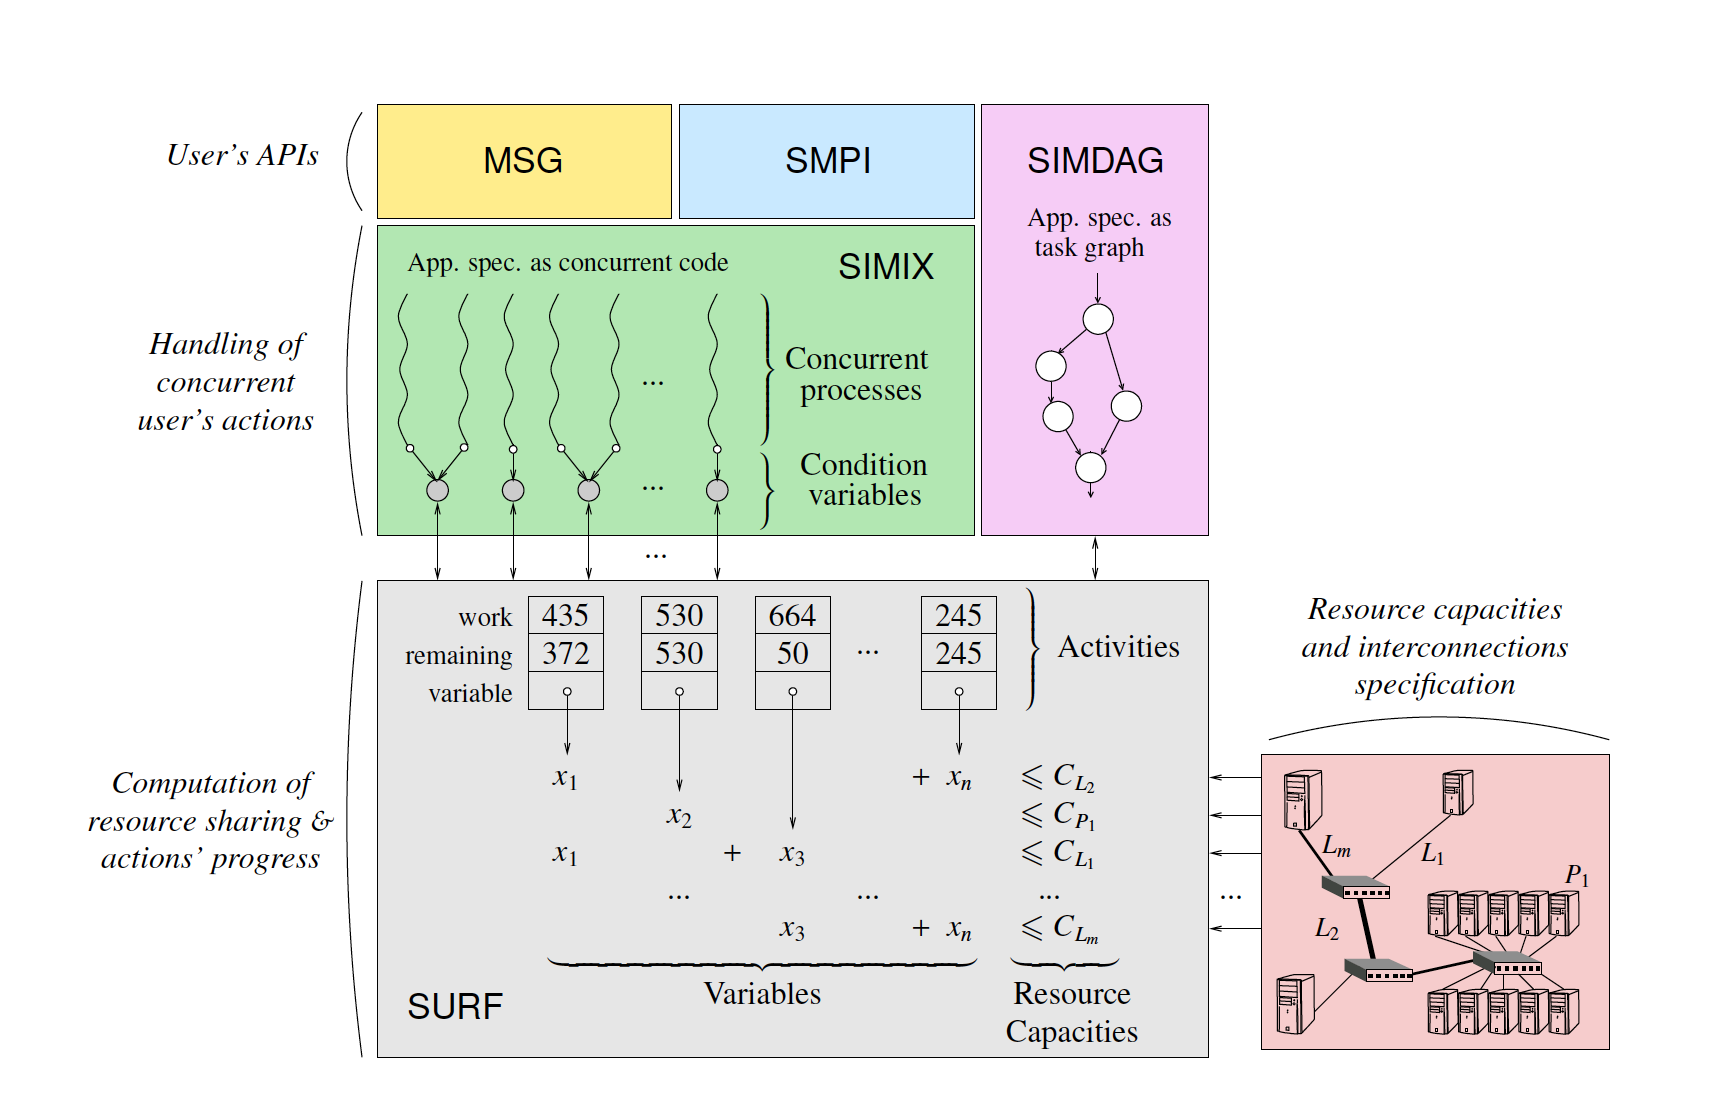
\includegraphics[width=\linewidth]{figures/simgrid.png}
%     \vspace*{-0.7cm}
     \caption{Overview and main components in \simgrid framework}
%     \vspace*{0.5cm}
     \label{fig:simgrid}
\end{figure*}

At the top are three APIs provided by \simgrid. 
The MSG API enables users to describe simulated applications as sets of 
concurrent processes. 
The SMPI API is also used to simulate applications as sets of 
concurrent processes, but these processes are automatically created from 
existing applications written in C or Fortran that uses the MPI standard.
The simulation mechanisms for the concurrent processes for MSG and SMPI APIs
are implemented as part of the SIMIX layer. It acts like a kernel that provides 
process control and synchronization abstractions by maintaining a set of 
condition variables.
The third API, SimDAG, does not use concurrent processes but instead 
allows users to specify abstract task graphs of communicating computational 
tasks with non-cyclic dependencies.
The simulation core that simulates the execution of activities on resources, 
is called SURF and is shown at the bottom of the figure.
Each application activity is described by the amount of remaining workload 
and the total amount of workload on resources.
An activity finishes when it reaches zero amount of remaining workload and 
signals SIMIX with corresponding condition variables. 
 
Throughout its history, \simgrid has been developed with the goal 
to improve both accuracy and scalability. 
The framework uses a unified model for the simulation of the execution 
of activities on simulated resources.
This model is purely analytical so as to afford scalability by avoiding cycle-, 
block-, and packet-level simulation of compute, storage, and network 
resource usage \cite{casanova2014simgrid}.
In the past years, \simgrid has also been the object of many invalidation and 
validation studies \cite{bedaride2013toward,velho2013validity,
velho2009accuracy,lebre2015}, and its simulation models 
have been shown to provide compelling advantages over other simulation 
frameworks in terms of both accuracy and scalability.

\subsubsection{WRENCH framework}

Several studies acknowledge that the popular \simgrid framework
offers compelling capabilities in terms of scalability and simulation accuracy.
Nevertheless, due to the low-level API, using \simgrid to implement 
a simulator of a complex system is extremely labor-intensive~\cite{kecskemeti_2014}. 
For that reason, \wrench ~\cite{casanova2020fgcs}, a framework for 
simulation of Workflow Management Systems (WMSs), has been developed 
to provide convenient, reusable, high-level abstractions that build on 
SimGrid to benefit from its scalable and accurate simulation models.
\wrench was not developed as a simulator but as a simulation framework 
distributed as a C++ library. 

\begin{figure*}[!h]
     \centering
     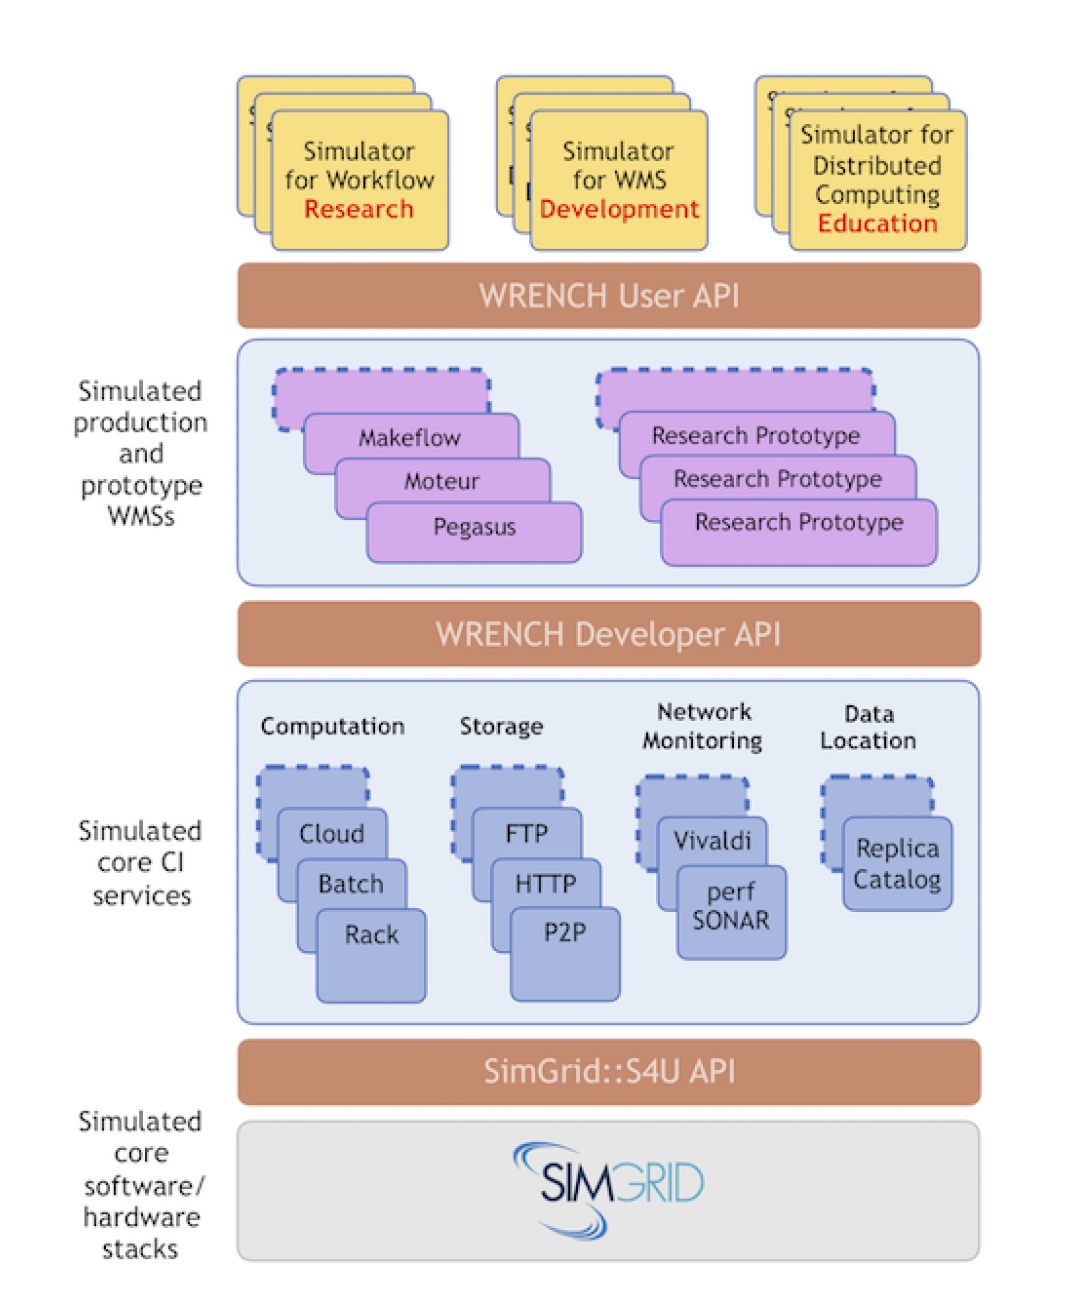
\includegraphics[width=0.75\linewidth]{figures/wrench.png}
%     \vspace*{-0.7cm}
     \caption{The four layers in the \wrench architecture from bottom 
     to top: simulation core, simulated core services, 
     simulated WMS implementations, and simulators.}
%     \vspace*{0.5cm}
     \label{fig:wrench}
\end{figure*}

Figure~\ref{fig:wrench} extracted from ~\cite{casanova2018wrench} 
shows the software architecture of \wrench. 
At the bottom level is \simgrid, the simulation core, which is responsible for 
simulating low-level software and hardware stacks.
The next layer implements CI services (abstractions for simulated 
cyberinfrastructure), that are commonly found in distributed platforms.
Currently, WRENCH provides services in 4 categories: 
\textit{compute services} that provide access to compute resources to 
execute applications; 
\textit{storage services} that provide access to storage resources for 
storing data data; 
\textit{network monitoring services} that can be queried to
determine network distances; and 
\textit{data registry services} that can be used to track the data location.
The above layer in the software architecture includes simulated WMSs, 
which interact with the CI services in the lower layer using the WRENCH 
Developer API.
Finally, the top layer consists of simulators that configure and instantiate 
CI services and WMSs on a given simulated hardware platform, that launch
simulation, and that analyze the simulation output.

\subsubsection{Why \simgrid and \wrench?}

In this work, we use the \simgrid and \wrench simulation
frameworks to implement a page cache simulation model.  
The high accuracy of \simgrid achieved with a set of state-of-the-art 
macroscopic simulation models was demonstrated by (in)validation studies 
and comparisons to competing frameworks~\cite{smpi_validity, 
velhoTOMACS2013, simutool_09, nstools_07, lebre2015, 
pouilloux:hal-01197274, smpi_tpds2017,  7885814, 8048921, 7384330}.  
But one significant drawback of \simgrid is that its simulation
abstractions are low-level, meaning that implementing a
simulator of complex systems can be labor-intensive. 
To remedy this problem, we targeted \wrench because it is a recent,
actively developed framework that provides convenient higher-level 
simulation abstractions so that simulators of complex applications and
systems can be implemented with a few hundred lines because it is extensible, 
and because it reuses \simgrid's scalable and accurate models.